\documentclass[11pt, a4paper]{article}

\usepackage[utf8]{inputenc}
\usepackage[french]{babel}
\usepackage[T1]{fontenc}
\usepackage{sistyle}
\usepackage{graphicx}
\usepackage{url}

\usepackage{listings}
\usepackage{color}
\definecolor{mygreen}{rgb}{0,0.6,0}
\definecolor{mygray}{rgb}{0.5,0.5,0.5}
\definecolor{mymauve}{rgb}{0.58,0,0.82}
\lstset{ %
  backgroundcolor=\color{white},   % choose the background color
  basicstyle=\footnotesize,        % size of fonts used for the code
  breaklines=true,                 % automatic line breaking only at whitespace
  captionpos=b,                    % sets the caption-position to bottom
  commentstyle=\color{mygreen},    % comment style
  escapeinside={\%*}{*)},          % if you want to add LaTeX within your code
  keywordstyle=\color{blue},       % keyword style
  stringstyle=\color{mymauve},     % string literal style
}

\usepackage[left=2.5cm,right=2.5cm,top=2.5cm,bottom=2.5cm]{geometry}

\bibliographystyle{plain}

\title{Programmation parallèle avec des Acteurs \\ \large{Projet de session INF7845 \\ UQAM}}
\date{\today}
\author{Antoine Laurent}

%\linespread{1.5}

\begin{document}
\maketitle\thispagestyle{empty}
\newpage 
\tableofcontents
\listoffigures
\newpage
\
\section{Introduction}
La concurrence est le fait de pouvoir exécuter des programmes, ou des fonctionnalités de ce programme en parallèle. Ce qui permet d'avoir plus de puissance de calcul ou moins d'attente lors de requêtes bloquantes.
\par Le modèle acteur est un modèle inventé par Hewitt \cite{hewitt1973session}. La programmation par acteur est utilisée pour sa facilité de faire de la concurrence, on peut retrouver des applications de mails, où chaque acteur identifie une boite mail et envoie des mails aux adresses des autres acteurs. Mais on l'utilise aussi pour faire des applications réactives ou encore des applications du cloud, par exemple la messagerie de Facebook était écrite en Erlang, qui est un langage acteur \cite{agha2014actors}. Twitter aussi utilise le modèle acteur avec Scala \cite{twitter_concurency}. Aussi, on peut voir que Microsoft utilise la programmation acteur pour  sa librairie de concurrence par agents.\cite{micr_concurency}
\par En ce qui concerne les langages de programmation, on retrouve Erlang qui implémente son modèle de concurrence de façon acteur, Scala qui permet la programmation acteur grâce à la librairie de Akka. Akka est une bibliothèque qui permet d'avoir le modèle acteur pour la JVM. On peut retrouver Ruby avec celluloid, Python avec Pykka, Nit et encore d'autres langages.

\section{Le modèle Acteur théorique}

Dans cette partie on va introduire le modèle théorique des Acteurs, c'est à dire ce que sont les Acteurs et comment Hewitt a pensé ce modèle quand il l'a introduit en 1973 \cite{hewitt1973session}. Pour cela on va voir la définition d'un Acteur, ce qu'ils peuvent faire comme actions et l'encapsulation de leur état interne. Ensuite on regardera comment ils communiquent entre eux et comment ils introduisent l'indéterminisme. Puis on s'intéressera à comment les acteurs sont résistants aux pannes. Pour enfin voir le cycle de vie d'un Acteur.

\subsection{Qu'est ce qu'un Acteur}

Comme pour la programmation objet d'Alan Key où tout est objet, les objets ayant leur propre mémoire et ils communiquent par message, dans le modèle Acteur de Hewitt, tout est acteur, les acteurs encapsulent leur état interne et ils communiquent par message. Hors les objets sont synchrones alors que les acteurs envoient les messages de manière asynchrone. 
\par 
Un acteur est donc une entité qui, à la réception d'un message peut: 
\begin{itemize}
\item Envoyer des messages à lui-même ou à d'autres acteurs. Ces messages sont émis de manière asynchrone.
\item Changer de comportement : il effectue une action liée à ce message et peut définir son comportement au prochain message.
\item Créer un nombre fini de nouveaux Acteurs.
\end{itemize}
On verra après que l'habilité de l'Acteur d'être asynchrone, de pouvoir créer de nouveaux acteurs et de protéger son état interne permet de faire de la parallélisation très facilement et d'avoir une mise à l'échelle simplifiée.

\subsection{Communication}

Comme dit plus haut les Acteurs communiquent entre eux par messages. Dans le modèle acteur, il n'y a pas de canaux de communication à établir (comme un pipe pour les forks). Les acteurs communiquent d'eux-même, soit par le réseau si le système est distribué sur plusieurs machines, soit en interne lorsqu'ils sont présents sur la même machine. De plus la stratégie d'envoi de messages est la technique du meilleur effort. Il n'y a pas de réémission, c'est-à-dire que lorsqu'un Acteur envoie un message à un autre, celui-ci recevra le message au plus une fois. 
\par Ces messages sont adressés aux différents Acteurs par leurs adresses. En effet un acteur peut être associé à une ou plusieurs adresses et on peut noter aussi que plusieurs Acteurs peuvent avoir la même adresse. Un bon exemple pour schématiser cela est de penser au moteur de recherche Google, on connaît tous une seule adresse de Google, pourtant on n'effectue pas tous nos recherches sur le même serveur.
\par Les Acteurs ont une boite aux lettres, (mailbox) dans laquelle ils reçoivent les messages qui leur sont adressés. Cela marche un peu à la façon du système de poste si l'on veut s'en faire une image. Un acteur envoie un message et il est reçu dans la boite aux lettres de l'acteur concerné. Ils traitent alors un message reçu à la fois.
\par Il est important aussi de noter que le temps que va mettre un message à arriver à destination n'est pas connu. L'ordre d'arrivée des messages est donc complètement indéterminé. Ceci amène la propriété de l'indéterminisme au modèle Acteur. En effet si on reprend l'exemple de Hewitt \cite{video_hewitt}, on imagine qu'un acteur s'envoie à lui même un message <<go>> et un message <<stop>> comme décrit figure \ref{fig1}. À la réception du message <<go>> l'acteur incrémente un compteur et à la réception du message <<stop>>, il arrête de compter. Étant donné que l'on ne sait pas combien de temps vont mettre les messages à revenir à l'acteur, et que ça ne dépend pas du système, le nombre obtenu à la réception du message <<stop>> est complètement aléatoire. Le modèle acteur a donc de l'indéterminisme.

\begin{figure}
\center
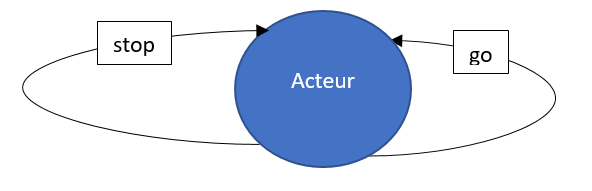
\includegraphics[scale=0.5]{actor_underminisism}
\caption{Exemple de l'indéterminisme du modèle Acteur.}
\label{fig1}
\end{figure}

\subsection{Concurrence avec les Acteurs}
Un des avantages principal du modèle Acteur est le fait qu'il introduit au programmeur de la concurrence à haut niveau. Dans le monde de la concurrence on peut retrouver deux manières de synchroniser les programmes, soit avec des états partagés comme les threads, soit avec des messages, comme pour les Acteurs \cite{haller2012actors}. Les threads peuvent devenir très vite difficile à programmer, à cause des verrous mortels, des courses à la donnée (data race). En effet ils utilisent des états partagés pour faire leurs calculs et cela oblige le programmeur à bien réfléchir à comment les threads vont communiquer et à quels moments protéger les variables partagées. Cela oblige à passer plus de temps à réfléchir à comment éviter les conflits entre les threads que de regarder la concurrence à un plus haut niveau. C'est à dire que l'application se déroule bien, de manière la plus efficace possible.

\par Les Acteurs eux ne possèdent pas d'états partagés, en effet chaque acteur a son propre état interne, et il ne doit pas communiquer d'état par messages par référence aux autres acteurs ou à lui même. Car s'il faisait ça on retomberait sur un problème de verrou mortel ou de course à la donnée. Le fait de communiquer par message empêche toute sorte de verrou mortel ou de course à la donnée. En effet une course arrive lorsque deux threads accèdent à la même donnée et au moins un des accès change la donnée \cite{haller2012actors}. On ne peut pas avoir ça avec les systèmes de messages, mais des courses à la donnée de plus haut niveau peuvent arriver. Par exemple, on a vu qu'on ne sait pas l'ordre d'arrivée des messages, et dans le cas d'une transaction bancaire par exemple, si deux acteurs envoient un message à un troisième qui est la banque pour demander un retrait. Alors si la banque n'a assez d'argent que pour un seul des acteurs, le premier message qu'elle va recevoir va avoir son argent alors que le deuxième non. Et cela indépendamment de l'ordre d'envoi des messages. 

\par De plus on peut voir que les acteurs sont beaucoup plus légers que les threads. Ils peuvent être plus facilement créés et détruits. On peut donc en créer beaucoup plus. De plus sur la JVM (Java Virtual Machine) par exemple, les threads sont des processus plus lourds car ils sont créés pour utiliser toute la puissance du processeur de la JVM. Et alors qu'on va pouvoir créer quelques milliers de threads en parallèle sur la JVM, on va pouvoir y créer des millions d'acteurs. \cite{haller2012actors}.
\par Le fait de pouvoir créer plus facilement des acteurs que des threads, et en plus grand nombre, ainsi que de pouvoir étendre la puissance horizontalement (sur un réseau de machine), rend la mise à l'échelle très efficace comparé aux threads classiques. Un inconvénient de la concurrence par messages peut être la consommation importante que ça va engendrer au niveau du canal de communication.

\subsection{Tolérance aux pannes}
Le modèle Acteur a comme autre propriété d'être tolérant aux pannes, de la même façon qu'Erlang (qui est un langage de programmation basé sur le modèle Acteur) et sa philosophie <<Let it crash>>. Donc si un acteur venait à lancer une exception, il ne mettrait pas en danger tout le système, mais l'erreur serait alors envoyée à un superviseur qui déciderait de le relancer l'acteur, ou de l’arrêter.
\par Cela est possible car comme dit plus haut aucun acteur ne partage d'état avec d'autres acteurs du programme, il ne met donc pas en danger les autres acteurs lorsqu'il lui arrive une erreur.
\par On a donc chaque acteur qui est supervisé par un autre acteur appelé superviseur, mais on peut alors se demander : <<qui supervise le superviseur>>. L'idée est alors d'avoir une sorte de hiérarchie de superviseurs, qui vont chacun superviser un ou plusieurs superviseurs de plus bas niveau, et ainsi pouvoir récupérer leurs erreurs. Au sommet de la hiérarchie se trouverait le superviseur racine qui lui supervise le thread principal, comme par exemple Akka l'a implémenté \cite{akka}.

\subsection{Les Acteurs dans le monde actuel}
Aujourd'hui on peut retrouver des bibliothèques qui permettent d'implémenter le modèle acteur sur différents langages de programmation, comme Akka, Celluloid ou encore la bibliothèque Acteur de Nit. Bibliothèques que l'on verra dans la suite de ce document. Mais il existe aussi des langages qui ont été créés par rapport à cette conception des acteurs. On peut retrouver Erlang qui est très orienté Acteur, mais ou on n'a pas chaque entité qui est un acteur, en effet il existe des types durs comme <<int>>, <<char>>, etc. On peut aussi parler d’Elixir, qui fait l'objet d'une étude pour ce travail de session.
\par En plus des langages de programmation, le modèle acteur est utilisé dans le web et le cloud \cite{agha2014actors,vecchiola2009high}. Par exemple on peut citer l'application de messagerie de Facebook qui était anciennement écrite en langage acteur, ou Twitter qui est développé en Scala, et dont le modèle de concurrence est un modèle acteur \cite{twitter_concurency}. Pour citer des projets plus récents, le service en ligne du jeu Halo 4 est implémenté en acteur, avec le framework Orleans développé par Microsoft.

\section{Différentes bibliothèques qui implémentent les Acteurs}
Dans cette partie on va regarder les deux bibliothèques suivantes : Akka pour la JVM et la bibliothèque Acteur de Nit. On va regarder comment utiliser les acteurs dans ces bibliothèques et comment elles implémentent le modèle Acteur. Plus tard dans le document on parlera des avantages et des faiblesses de chacune d'elles, mais cette partie est consacrée à l'expérimentation des bibliothèques. 
\par Pour cela on va commencer par regarder la bibliothèque Akka, qui est la plus grosse des deux et permet de se rapprocher le plus du modèle Acteur. Et enfin on regardera la bibliothèque de Nit, qui est basée sur celle de Celluloid.

\subsection{Les acteurs en Scala avec Akka}
Akka est une bibliothèque qui apporte le modèle Acteur à la JVM. Dans le cadre de ce projet de session on va regarder seulement Akka pour le langage de programmation Scala, car il parait plus simple à première vue de programmer en acteur avec Scala qu'avec le langage Java. C'est une bibliothèque écrite en Scala et elle a pour but, en plus d'implémenter le modèle Acteur, de permettre au développeur de fournir un code plus simple, performant et fiable par rapport à la bibliothèque concurrente de base de Scala, ou de Java.

\subsubsection{Implémentation des Acteur par références}
Les acteurs dans Akka peuvent être désignés de deux manières différentes : par leur référence (\texttt{ActorRef})ou par leur chemin (\texttt{path}). Bien que les deux servent à désigner un acteur, les deux ne sont pas la même chose. 
\begin{itemize}
\item \textbf{Une référence :} c'est ce qui représente l'acteur créé et permet d'envoyer des messages à cet acteur. En effet lorsqu'on crée un acteur on obtient une référence qui est un sous-type de \texttt{ActorRef}. On ne peut pas créer un acteur en utilisant l'opérateur \texttt{new}, mais on doit utiliser \texttt{Props} qui est une classe de configuration pour créer des acteurs. On peut voir la création d'un acteur dans la figure \ref{act_crea}.
\par Le fait de ne pas pouvoir instancier directement un acteur avec un \texttt{new} permet de garantir de manipuler un acteur et de gérer l'envoi de messages. En effet il est alors impossible d'appeler une méthode que l'on définirait dans la classe de l'acteur. On a donc une abstraction qui permet de gérer avec ce qui semble de vrais acteurs. 
\item \textbf{Le chemin :} c'est le nom de l'acteur. Il est représenté par la suite successive de superviseur par lesquels on doit passer pour l'atteindre (sachant qu'un superviseur est le père de l'acteur). Le \texttt{path} est différent de la référence, en effet la référence désigne un seul acteur alors que le chemin désigne un nom sous lequel il peut y avoir ou non un acteur.
\par Un \texttt{path} est local mais il peut aussi être un chemin à distance, par exemple le chemin de l'acteur de la figure \ref{act_crea} s'obtient par l'appel à la méthode \texttt{actor.path} et nous donne \texttt{akka://SimpleSystem/user/SimpleActor}. Un chemin à distance pourrait être \texttt{akka.tcp://my-sys@host.example.com:5678/user/service-b}
\newline
\end{itemize}
\par 
Pour créer les premiers acteurs dans Akka il faut avoir un système d'acteur, c'est lui qui va superviser les acteurs qui seront créés par lui. Pour créer un système d'acteur il suffit d'utiliser la fonction \texttt{ActorSystem("NomSystème")}. Ensuite chaque acteur que vous créez aura son propre contexte, et pourra créer des acteurs à partir de celui-ci. Il représente l'interface que l'on a avec l'acteur. 
\par Une fois que l'on a le système d'acteur, on peut créer et obtenir la référence sur l'acteur grâce à la méthode \texttt{actorOf()}. On peut alors commencer à envoyer des messages à cet acteur.

\begin{figure}[ht]
\centering
\begin{lstlisting}[language=Scala]
__________________________________________________________________________
  class SimpleActor extends Actor {
    def receive = {
      case s:String => println("String : "+s)
      case i:Int => println("Int : "+i)
    }
    
    def foo = println("method foo")
  }
  val system = ActorSystem("SimpleSystem")
  val actor = system.actorOf(Props[SimpleActor], "SimpleActor")
  
  actor ! "Hello"
___________________________________________________________________________
\end{lstlisting}
\caption{Création d'un Acteur en Scala avec Akka}
\label{act_crea}
\end{figure}

\subsubsection{Tolérance aux pannes}
Dans cette partie, on va aborder la tolérance aux pannes. On va regarder comment Akka implémente la philosophie <<Let it crash>>, quels sont les mécanismes et la philosophie employés. Pour cela on va voir qu'est-ce qu'un programme tolérant aux pannes devrait être capable de faire, et le comparer avec ce qu'Akka permet de faire. Ensuite on regardera comment Akka supervise les acteurs et les actions qu'il peut prendre et le cycle de vie d'un acteur. Pour enfin s’intéresser aux stratégies utilisées par le superviseur pour savoir quelle action faire lorsqu'un type d'erreur survient.
\par Pour étudier la tolérance aux pannes dans cette partie on se base principalement sur la documentation officielle d'Akka \cite{akka} et le livre Akka in Action \cite{roestenburg2015akka}.

\par Tout d'abord on va rappeler ce que veut dire d'être tolérant aux pannes. Être tolérant aux pannes ne veut pas dire que qu'aucune exception ne doit arriver dans le système et que rien ne doit jamais tomber en panne. Au contraire, c'est de savoir que des pannes arrivent toujours, mais d'essayer de conserver le système en ligne sans avoir d'erreurs graves en essayant de récupérer ces pannes. Souvent lorsqu'une panne arrive, il est seulement important que les principales fonctionnalités d'un programme restent disponibles, et on peut alors arrêter les plus petites si elles ont un problème, ou les mettre de coté pour trouver une solution plus tard. Si ces fonctionnalités sont trop importantes pour être arrêtées alors il est possible d'avoir une sauvegarde de ces fonctionnalités pour pouvoir les remplacer directement.

\par Parlons maintenant des bonnes stratégies que l'on devrait avoir lorsqu'on parle d'un programme tolérant aux pannes. Ce comportement idéal est reporté du livre Akka in Action \cite{roestenburg2015akka} et ses caractéristiques sont décrites dans le tableau \ref{table1}.
\newline

\begin{table}[h]
\centering
\begin{tabular}{|l|p{.7\textwidth}|}
\hline
Isoler la faute & Une faute ne doit pas faire tomber en panne le système et doit être isolée pour cela.\\ \hline
Structure & Le système doit avoir une structure pour isoler les éléments en erreur des éléments actifs. \\ \hline
Redondance & On doit pouvoir avoir un composant de secours quand le composant tombe en erreur.\\ \hline
Remplacement & On doit pouvoir remplacer un composant du système sans que les autres composants qui étaient en communication avec soient dérangés par ce changement. Ils doivent pouvoir communiquer avec le remplacement de la même façon qu'ils communiquaient avec l'ancien. \\ \hline
Redémarrage & On doit pouvoir redémarrer un composant à son état initial. \\ \hline
Cycle de vie & Les composant devront avoir un cycle de vie défini pour pouvoir être démarré, stoppé ou redémarré. \\ \hline
Suspension & Lorsqu'un composant est en erreur, les autres composants actifs doivent arrêter de communiquer avec. \\ \hline
Séparation du code & Le code pour l’exécution normale du programme ne doit pas être mélangé avec le code destiné au recouvrement de panne. \\ \hline
\end{tabular}
\caption{Caractéristiques pour un système tolérants aux pannes}
\label{table1}
\end{table}
\par On va maintenant s'intéresser à la gestion des pannes par Akka, pour pouvoir comparer avec le comportement idéal décrit dans la table \ref{table1}. Dans Akka le flux normal du programme est géré séparément du flux de recouvrement. Le flux normal correspond à l’exécution normale du programme, c'est-à-dire quand il n'y a pas d'erreur et le flux de recouvrement correspond à ce qui se passe quand l'acteur crash. Effectivement, les acteurs qui participent au flux normal sont juste programmés pour effectuer les tâches du programme. Ils jouent leur rôle d'acteur, et ce sont les superviseurs de ces acteurs qui sont prévenus lorsqu'il y a une erreur sur un acteur qu'ils supervisent qui crash. 
\newline
\textbf{Général :}
\par Quand un acteur crash, on le laisse crasher, on n'attrape pas l'exception. sa boite aux lettres est alors suspendue le temps que son superviseur choisisse une action à effectuer pour cet acteur. Le superviseur a alors 4 options vis-à-vis de l'acteur crashé :
\begin{itemize}
\item Redémarrer son subordonné, ce qui le fait revenir à son état initial.
\item Reprendre l’exécution du subordonné, il conserve alors son état interne.
\item Arrêter le subordonné.
\item Faire monter l'information lorsqu'il ne sait pas comment gérer l'erreur.
\end{itemize}
Lorsqu'on reprend l’exécution d'un acteur, on reprend l'exécution de tous les acteurs qu'il a créés. De même lorsqu'on redémarre cet acteur, on redémarre tous ses fils, en les ayants arrêtés préalablement.
\par Chaque acteur est supervisé par l'acteur qui le crée. En effet Akka a choisit un modèle de supervision parentale. Il n'y a pas d'adoption, si un parent est arrêté alors tous ses enfants le sont aussi. Cela permet un arrêt propre de tout un arbre ou sous arbre d'acteurs.
\newline
\newline
\textbf{Cycle de vie :}
Comme on l'a vu plus haut, un acteur peut être démarré, redémarré ou bien arrêté. C'est les trois types d’événements que l'on retrouve dans le cycle de vie d'un acteur dans Akka. Lors de l'arrêt d'un acteur, il ne peut plus recevoir de messages et il va se faire ramasser par le <<garbage collector>>.

\par On peut démarrer un acteur avec la méthode \verb!actorOf! qui est soit une méthode utilisée par le \verb!ActorSystem! si c'est un acteur créé dans le thread principal (un acteur de haut niveau). Soit une méthode utilisée par \verb!ActorContext! si c'est un acteur créé par un autre acteur du système. Une fois l'instance créée, la méthode \verb!preStart! est appelée, puis l'acteur est démarré. On peut utiliser cette méthode pour initialiser l'état de l'acteur.

\par On arrête un acteur en utilisant la méthode \verb!stop!, soit sur l'\verb!ActorSystem! ou sur l'\verb!ActorContext!. Comme pour le démarrage d'un acteur, avant qu'on termine l'acteur, la méthode \verb!preStop! est appelée. 	 

\par Enfin l'acteur est redémarré de base lorsqu'il crash, on verra cela dans la partie Superviseur et Stratégie. Par exemple si on envoie l'exception \texttt{throw new IllegalStateException( "restart forcé")} alors le superviseur fera redémarrer l'acteur. Quand un acteur crash, on remplace l'acteur par un nouvel acteur et on l'attache à sa référence \verb!ActorRef!. L'acteur crashé ne reçoit pas de message \verb!Terminate!, on peut donc lui faire envoyer un message à lui-même après le redémarrage. Ainsi le nouvel acteur recevra ce message puisque c'est lui qui est associé à l'\texttt{ActorRef}.
\newline
\newline
\textbf{Superviseur et Stratégies :}
Lorsque l'on démarre une application Akka, on démarre au moins trois acteurs, qui forment une hiérarchie (figure \ref{fig2}): 
\begin{itemize}
\item Le root Guardian : c'est le superviseur de tous les acteurs de haut niveau. Il ne peut pas faire remonter de messages, il n'a pas de superviseur, ce n'est donc pas un vrai acteur. Il arrête ses fils  au moindre trouble \cite{akka}, et c'est lui qui arrête le système d'acteur.
\item Le user Guardian : c'est le superviseur de tous les acteurs créés par l'utilisateur. Si on éteint cet acteur, on éteint tous les acteurs de l'utilisateur.
\item Le system Guardian : c'est le superviseur de tous les loggers de l'application.
\newline
\end{itemize}

\begin{figure}
\centering
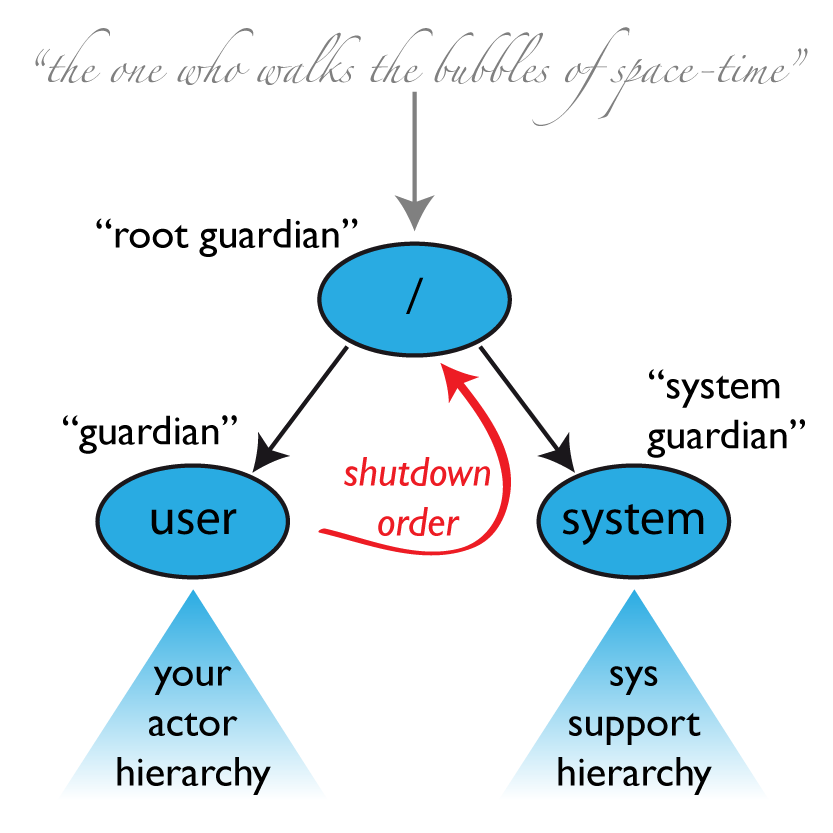
\includegraphics[scale=1]{guardians.png}
\caption{hiérarchie des trois superviseurs de plus haut niveau dans Akka \cite{akka}}
\label{fig2}
\end{figure}

\par Les acteurs qui supervisent ont une stratégie pour connaître  quelle action prendre quand une exception se produit. Par défaut un superviseur va vouloir redémarrer l'acteur en question pour tout type d'exception qui a produit le crash de l'acteur. Les seuls cas où il ne va pas essayer de redémarrer son fils et si l'erreur survient lors de l'initialisation de l'acteur ou lorsque celui-ci a été tué.
\par Cette stratégie peut être changée si on veut en redéfinissant la méthode \texttt{supervisorStrategy}. On peut voir un exemple de redéfinition figure \ref{fig3}.

\begin{figure}[ht]
  \begin{lstlisting}[language=scala]
  __________________________________________________________________________
  import akka.actor.OneForOneStrategy
  import akka.actor.SupervisorStrategy._
  import scala.concurrent.duration._

  override val supervisorStrategy =
      OneForOneStrategy(maxNrOfRetries = 10, withinTimeRange = 1 minute) {
        case _: ArithmeticException => Resume
        case _: NullPointerException => Restart
        case _: IllegalArgumentException => Stop
        case _: Exception => Escalate
  __________________________________________________________________________
  \end{lstlisting}
  \caption{Changement de stratégie pour un superviseur \cite{akka}}
  \label{fig3}
\end{figure}
\par On peut voir ici qu'on utilise la stratégie \texttt{OneForOneStrategy}, cela signifie qu'on différencie tous les fils lorsqu'on reçoit une exception de l'un d'eux. Les autres acteurs supervisés par l'acteur ne sont pas concernés par le destin de celui qui a crashé. Au contraire la stratégie \texttt{AllForOneStrategy} associe le même destin à tous les acteurs qu'il supervise. Si un acteur crash et que le superviseur le tue, alors tous les acteurs sont arrêtés.
\newline
\newline
\textbf{Monitoring :}
\par Un acteur ne peut pas être superviseur d'un autre acteur qu'il n'a pas créé, mais il peut être son moniteur grâce à la méthode \texttt{watch(ActorRef)}, qui est appelée sur l' \texttt{ActorContext}. Ainsi lorsque l'acteur est arrêté, le moniteur reçoit un message lui disant que l'acteur qu'il regardait s'est arrêté. C'est une des raisons pour laquelle ils ne peuvent pas tuer un acteur lorsqu'il le redémarre car sinon un acteur qui était son moniteur ne pourrait pas savoir s'il a été redémarré ou arrêté.
\newline
\par 
On a donc pu voir que Akka permet de respecter complètement les bonnes stratégies pour la tolérance aux pannes. En effet, on peut isoler la faute, pour cela un superviseur a juste à terminer l'acteur. On peut remplacer un acteur sans que le système soit affecté, ce qui implique une structure pour gérer l'acteur erroné et un remplacement fonctionnel. Cela convient aussi pour la redondance, en effet si un acteur peut être remplacé il peut alors être remplacé par une sauvegarde de lui-même. Un acteur a un cycle de vie et peut être suspendu. Enfin le code application est défini indépendamment du code pour la récupération d'erreurs.
\subsubsection{Messages et Boite aux lettres}
Akka nous donne des références sur des acteurs, et on peut envoyer des messages à ces références via la méthode \texttt{tell(message, ActorRef)} ou alors plus simplement avec le \texttt{!} comme montrer dans la figure \ref{act_crea}. Lorsqu'un acteur reçoit un message, il est réceptionné dans sa boite aux lettres, qui est implémentée comme une FIFO. Chaque acteur a généralement sa propre boite aux lettres, mais dans certains cas un groupe d'acteurs peut avoir la même boite aux lettres (voir BalancingPool \cite{akka}). De plus cette boite aux lettres peut être configurée sur plusieurs critères, elle peut par exemple bloquer l'arrivé de nouveaux messages si celle-ci est pleine, ou être partagée entre plusieurs acteurs comme énoncé ci-dessus.
\par Lorsqu'un acteur reçoit un message il fait ce qu'on appelle du message matching pour voir s'il a une action spécifiée à la réception de ce message. On peut voir par exemple dans la figure \ref{act_crea} que l'acteur sait comment réagir aux String et aux Integers. On peut aussi, dans le but de rendre l'application <<plus Acteur>>, créer des cas de messages en créant des objets Scala, comme on peut le voir dans la première ligne de la figure \ref{cas_mesg}.
\par Lorsqu'un message est envoyé mais ne peut pas joindre la destination parce que par exemple l'acteur est terminé, le message va dans ce qu'appelle Akka les DeadLetters, c'est une boite aux lettres où sont redirigés les messages qui ne peuvent pas être délivrés.
\par Akka, comme dans le modèle théorique n'assure pas la réception du message. En effet il sera reçu au plus une fois par le destinataire. Par contre Akka assure que si plusieurs messages sont envoyés à un acteur par l'envoyeur successivement, alors les messages seront reçus dans le même ordre que celui de l'envoi. Par exemple si A envoie à B m1, m2 et m3, alors si B reçoit m1, ce sera forcément avant m2 et m3.
\newline

\begin{figure}[ht]
\centering
\begin{lstlisting}[language=scala]
__________________________________________________________________________
case object AskNameMessage

class SimpleActor extends Actor {
  import context._
  implicit val timeout = Timeout(FiniteDuration(1, TimeUnit.SECONDS))
  
	def receive = {
	  case AskNameMessage => sender ! "Antoine"
	  case _ => context.actorSelection("akka://SimpleSystem/user/SimpleActor2").resolveOne().onComplete {
	    case Success(actorRef) => actorRef ! "coucou"
	    case Failure(ex) => println("user/" + "somename" + " does not exist")
	  }
	}
}
__________________________________________________________________________
\end{lstlisting}
\caption{Exemple de cas de messages et réception de tous messages en Scala avec Akka}
\label{cas_mesg}
\end{figure}

\par En plus de pouvoir envoyer un message de manière asynchrone avec la méthode \texttt{tell(...)}, Akka permet d'enregistrer ce message dans un Future avec la méthode \texttt{ask(mesg, Actorref)} ou encore \texttt{?}. Cela permet d'envoyer un message et d'attendre pour une réponse sans bloquer le thread principal. On peut ensuite récupérer ce résultat de manière bloquante, i.e en attendant que le future ai fini son exécution ou alors avec la commande \texttt{onComplete()}. On peut voir un exemple d'utilisation des futurs dans la figure \ref{futur}
\newline 

\begin{figure}[ht]
\centering
\begin{lstlisting}[language=scala]
__________________________________________________________________________
object future extends App {

	val system = ActorSystem("SimpleSystem")
	val myActor = system.actorOf(Props[SimpleActor], name = "myActor")

	implicit val timeout = Timeout(5 seconds)
	val future = myActor ? AskNameMessage
	val result = Await.result(future, timeout.duration).asInstanceOf[String]
	println(result)

	system.terminate()

}
__________________________________________________________________________
\end{lstlisting}
\caption{Exemple d'utilisation de Future dans Scala avec Akka}
\label{futur}
\end{figure}

\par Enfin on peut parler des routeurs qui permettent dans Akka d'implémenter le fait que plusieurs acteurs aient la même adresse. Ce n'est pas à proprement parler plusieurs acteurs avec la même adresse. On a un Routeur, qui est un acteur avec une adresse, ce routeur crée un Pool d'acteurs et lorsqu'il va recevoir un message, va pouvoir l'envoyer aux autres. La manière dont il l'envoie (broadcast, etc) dépend du protocole de routage qu'on lui demande d'implémenter.

\subsubsection{Autres fonctionnalités d'akka}
Akka est une très grande bibliothèque dans laquelle il existe beaucoup d'autres fonctionnalités. J'ai choisi ici d'essayer de présenter les fonctionnalités les plus importantes pour un système d'acteur mais aussi de comprendre comment elles ont été faites. Mais Akka est tellement large qu'on pourrait y consacrer un projet de session entièrement. Néanmoins je voulais mentionner quelques autres fonctionnalités, comme les clusters, la gestion de HTTP pour des applications Client Serveur, Actor DSL qui est une manière plus simple et rapide de faire de la programmation acteur. Toutes ces fonctionnalités peuvent être retrouvées dans la documentation d'Akka \cite{akka}.

%\subsection{Les acteurs en Ruby avec Celluloid}
%Dans cette partie 
%\subsubsection{Implémentations des acteurs}

%\subsubsection{Les Pools}

%\subsubsection{Tolérance aux pannes}

%\subsubsection{Cycle de vie}

\subsection{Les acteurs en Nit avec la bibliothèque d'acteur}
On va regarder dans cette partie comment est implémenté le modèle acteur dans le langage de programmation Nit et en quoi cela diffère d'Akka. Pour cela on regardera comment sont créer les acteurs, leurs caractéristiques et l'envoi de messages. On regardera aussi un exemple pour comprendre l’instanciation d'un acteur.

\subsubsection{Implémentations des acteurs}
L'implémentation diffère de celle d'Akka ici. En effet dans Akka un acteur était désigné par sa référence et avait une addresse. On pouvait alors manipuler <<directement>> cet acteur par le biais de la référence. Ici on distingue trois entités différentes :
\newline
\begin{itemize}
\item la classe qu'on veut faire devenir acteur
\item le proxy de cette classe. C'est lui qui va faire passer les messages à l'acteur.
\item l'acteur de la classe. C'est lui qui va recevoir les messages et les traiter.\\
\end{itemize}
\par 
Les messages correspondent aux différentes méthodes qui se trouvent dans la classe de base. Ces méthodes sont ensuite invoquées par l'acteur lorsqu'il a reçu et traite le message. Les messages suivent la propriétés des messages dans le modèle acteurs, c'est-à-dire qu'ils sont envoyés de manière asynchrone à l'acteur, les Acteurs étant des threads. Pour illustrer le modèle d'acteur de Nit, on peut regarder la figure \ref{acteur_nit}.
\par 
Pour ce qui est des caractéristiques des Acteurs dans Nit, on retrouve :

\begin{itemize}
\item Une boite aux lettres : elle est implémentée avec une collection concurrente. Elle permet d'ajouter des messages en fin ou au début de la collection avec les commandes \texttt{push, unshift} respectivement. Mais aussi de lire le premier message avec \texttt{shift}. On utilise une collection concurrente pour permettre de bloquer lors de toute opération de lecture ou d'écriture.
\item l'instance de l'objet qu'il représente : cet attribut est utilisé lorsque l'acteur reçoit un message, il appelle alors la méthode qui correspond au message sur l'instance qu'il représente.
\end{itemize}
On peut voir que contrairement aux propriétés du modèle acteur théorique, un acteur ici n'a pas d'adresse. C'est toujours son proxy qui va lui transmettre les messages. Un acteur ne peut pas non plus répondre à un message reçu de son proxy, car il ne peut pas envoyer de message. C'est l'instance qui demande l'envoi de messages asynchrones. Un acteur sert dans Nit un rôle purement concurrent.

\begin{figure}
\centering
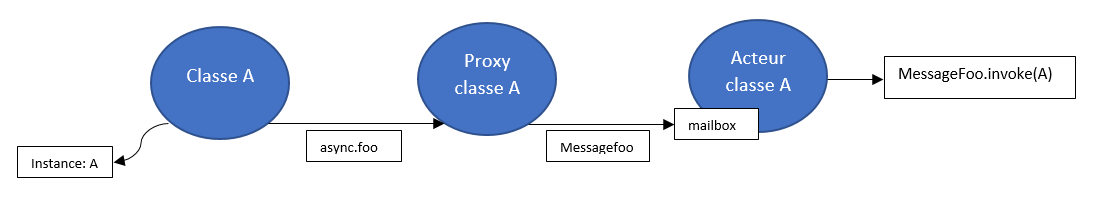
\includegraphics[scale=0.5]{acteur_nit}
\caption{\label{acteur_nit}Structure du modèle Acteur dans Nit }
\end{figure}

\subsubsection{Création d'un acteur dans Nit}
\par Un acteur est créé lors du premier appel une méthode avec le mot clé \texttt{async} devant la méthode. Par exemple \texttt{async.foo}, va d'abord créer le Proxy de cette classe, il crée à son tour l'acteur de la classe et lui envoie le message. L'acteur va alors exister jusqu'à l'arrêt du programme et des taches en cours par les acteurs ou jusqu'à ce qu'on le termine. On verra se procéder dans la supervision des acteurs.
\par Pour spécifier qu'une classe sera acteur on l'annote en utilisant le mot clé \texttt{acteur} après sa déclaration. On peut voir un exemple dans la figure \ref{nit_prog}

\subsubsection{Messages dans ce modèle d'acteur}

\par Dans la bibliothèque la classe peut être utilisée aussi bien en tant qu'acteur qu'en classe normale. En effet les appels des méthodes qui déterminenr si ça va être une exécution normale ou asynchrone par le biais d'un acteur. On distingue alors l'envoi de messages asynchrones aux acteurs par l'utilisation du mot clé \texttt{async} devant l'appel de la méthode.
\par Lors de l’exécution, chaque méthode qui se trouve dans l'objet instancier et annoté par le mot clé acteur est traduit en une classe Message, \texttt{MessageFoo} par exemple. Chaque message de méthode hérite lui de la classe des messages de la classe annotée <<acteur>>.
\par Donc lors de la première exécution asynchrone d'une méthode, on crée le proxy de cette classe, qui lui va associer chaque méthode à son message, créer l'acteur et lui envoyer le message dans sa boite aux lettres. L'acteur regarde en permanence pour des nouveaux messages dans sa boite aux lettres.
\par Les messages ont une méthode unique qui est \texttt{invoke(instance)}. Elle permet à l'acteur d'invoquer la méthode qui correspond au message sur l'instance qui l'a appelé, cela par l'acteur. Qui pour chaque message $m$ appelle \texttt{m.invoke(instance)}.
\par Ainsi par la propriété des objets et à condition que la variable ne soit pas accessible publiquement, on garde la propriété d'un état protégé et on évite les verrous mortels car les messages sont traités les uns à la suite des autres.

\subsubsection{Supervision et cycle de vie des acteurs}
Dans le modèle de Nit il n'y a pas vraiment de superviseur. On retrouve néanmoins le système qui connait tous les acteurs, et qui va attendre que la liste d'acteur soit vide, qu'ils aient tous finis de traiter leurs messages pour que le programme puisse quitter. Sinon l'appel à la méthode \texttt{active\_actors.is\_empty} est bloquant.
\par 
Il est possible de terminer la vie d'un acteur en lui envoyant les messages \texttt{terminate} qui va attendre que l'acteur ait fini de traiter ces messages, ou \texttt{terminate\_now} qui passe le message en premier et arrête l'acteur.

\subsubsection{Exemple simple}

Dans les figures \ref{nit_prog} et \ref{nit_prog_gen} on peut voir un programme simple qui a pour but de montrer comment fonctionne le modèle acteur dans Nit. On peut voir qu'on annote la classe A avec le mot clé acteur. Dans figure \ref{nit_prog_gen} on voit que Nit a créé deux messages un message qui représente tous les messages possibles de la classe A et un autre spécifique à la méthode \texttt{foo}. De plus on crée le proxy et l'acteur spécifique à la classe (l'acteur spécifique à A n'est pas présent sur cet exemple) et on associe l'acteur au proxy et l'envoi du message \texttt{AMessageFoo} à la méthode \texttt{foo}.

\begin{figure}
\centering
\begin{minipage}{.5\textwidth}
  \centering
  \begin{lstlisting}[language=ruby]
__________________________________________________________________________
class A 
        actor

        fun foo do print "foo"
end

var a = new A
a.foo
a.async.foo
__________________________________________________________________________
\end{lstlisting}
  \caption{Un exemple de programme utilisant les acteurs dans Nit}
  \label{nit_prog}
\end{minipage}%
\begin{minipage}{.5\textwidth}
  \centering
\begin{lstlisting}[language=ruby]
__________________________________________________________________________
####### Redef classes #######
redef class A
	redef var async is lazy do return new ProxyA.proxy(self)
end
####### Messages classes #######
class MessageA
	super Message
	redef type E: A
end

class AMessagefoo
	super MessageA
	redef fun invoke(instance) do instance.foo
end

####### Proxy classes #######
redef class ProxyA

	redef type E: ActorA
	#var actor: ActorA is noinit

	init proxy(base_class: A) do
		actor = new ActorA(base_class)
		actor.start
	end

	redef fun foo do
		var msg = new AMessagefoo
		actor.mailbox.push(msg)
	end
end
__________________________________________________________________________
\end{lstlisting} 
\caption{Le fichier générer par nit lors de l'exécution du programme Figure \ref{nit_prog}}
  \label{nit_prog_gen}
\end{minipage}
\end{figure}
%minipage test.nit

\section{Les avantages et faiblesses de ces bibliothèques}
On discutera dans cette partie des avantages et inconvénients de chaque bibliothèque. On regardera ce qu'elles implémentent par rapport au modèle acteur théorique. Ce qu'elles permettent de faire et ce qu'elles ne permettent pas.

\subsection{Akka}

\subsubsection{Avantages}
Akka est une bibliothèque qui implémente tous les principes fondamentaux du modèle acteur théorique. En effet lorsqu'on manipule des acteurs, on a l'impression de manipuler l'objet acteur en question bien que la bibliothèque soit implémentée par-dessus le paradigme de la programmation orientée objet. C'est rendu possible par le fait qu'on a accès à seulement une référence à notre classe, et que cette classe n'est pas instanciable à la façon objet.
\par La gestion de messages est elle aussi bien faite, en effet il est facile de dire à notre acteur que faire lorsqu'il reçoit un message, et comment en envoyer un autre. De plus chaque acteur ayant une adresse représentée par l'\texttt{actorRef}, il est facile d'envoyer un message à un autre acteur dont on connaît l'emplacement.
\par Il implémente le fait que des acteurs peuvent être sur des réseaux distincts mais communiquer quand même à travers TCP ou des websocket par exemple, ce qui rend la mise à l'échelle horizontale facile.
\par Akka met en place beaucoup de choses du modèle acteur et plus comme les superviseurs, qui permettent de gérer la tolérance aux pannes, ou encore les routers qui permettent de gérer le routage entre un master et ses workers. On peut noter aussi qu'il intègre toute la partie web et HTTP. 
\par Il est donc assez simple de raisonner en acteurs avec la bibliothèques Akka
\subsubsection{Inconvénients}
Un des plus gros désavantages d'Akka selon moi est que le fait d'implémenter toutes ces fonctionnalités rend le code assez complexe lorsque l'application devient grosse. Les acteurs communiquent entre eux par protocoles de messages et plus l'application devient grosse, plus ont a de risques de faire des courses à la donnée. 
\par Le fait qu'il y ait beaucoup de couches pour implémenter le modèle rend le débogage d'autant plus difficile. En effet on se retrouve souvent avec des exceptions assez importantes, qui peuvent être assez difficiles à comprendre et donc à comprendre d’où le problème vient.
\par Un autre problème est que les messages ne sont pas typés. On peut envoyer n'importe quel message à n'importe quel acteur et donc cela nécessite plus de test. On peut toujours faire du pattern matching sur les messages qui arrivent, mais si on oublie de spécifier un message le compilateur ne le verra pas.
\par Aussi le programmeur peut faire des anti-patterns qui cassent le modèle acteur, comme définir une variable globale à laquelle tous les acteurs vont pouvoir accéder et modifier. C'est une mauvaise idée car on va devoir verrouiller cette variable, et on retombe sur le problème de verrou mortel des threads.

\subsection{Nit}

\subsubsection{Avantages}
Bien que la bibliothèque de Nit pour les acteurs soit plus simple et petite, elle implémente le fait d'avoir un état partagé et de recevoir des messages. Elle convient donc très bien pour faire de la concurrence puisque les variables d'une instance de classe peuvent être privées.
\par De plus on peut écrire tout le code à la manière objet et le paralléliser avec des acteurs en ajoutant l'annotation \texttt{actor}. Cela rend l'utilisation d'acteur plus simple que dans Akka, lorsqu'on veut faire de la concurrence seulement.
\par Les messages sont typés puisqu'ils correspondent à des méthodes, et un acteur ne peut recevoir que des messages du type qui ont été définis dans la classe annotée acteur. 
\subsubsection{Inconvénients}
\par Les acteurs n'ont pas d'adresse, on ne peut donc pas envoyer de message d'un acteur à un autre acteur, et les applications comme celles du chat sont pas possibles si on raisonne en acteurs.
\par Il n'implémente pas le modèle acteur dans sa totalité mais permet de faire de la concurrence sans se soucier des verrous, et ce tant que l'on ne fait pas d'anti-pattern.

\section{Programme réalisé}
Dans ce projet de session j'ai été amené à tester les différentes bibliothèques qui permettent de faire de la programmation Acteur. Pour concrétiser cet apprentissage j'ai donc choisi de réaliser deux programmes, un qui est basé sur de la concurrence d'entré et sortie, et l'autre sur le calcul. 
\par Tous les programmes réalisés peuvent être trouvés sur le Github suivant \url{https://github.com/Drayer34/POO/tree/master/projet_session/programmes}.
\subsection{Mandelbrot}
J'ai décidé, pour le programme CPU-bounded, de réaliser le calcul de Mandelbrot, d'une part car c'est un calcul qui est facilement parallélisable et que j'avais déjà implémenté une version en Java avec des threads et aussi CUDA, qui se base sur le GPU. Il m'a donc été possible de voir si le modèle acteur était plus performant, ou du moins aussi performant que le modèle basé sur les threads.
\par 
Pour cela j'utilise un acteur \texttt{Master} qui va créer un nombre d'acteur \texttt{Worker} qu'il veut (ce sera le nombre de threads). J'ai divisé l'écran à calculer en barre verticale et chaque acteur calculera une barre verticale puis enverra son résultat au \texttt{Master}.
\par Une fois toutes les parties récupérées, on affiche le résultat.
\newline
\par Niveau performance, on voit que plus on va avoir d'acteurs plus on va calculer vite la fractale Mandelbrot, mais que comparé à la version à Threads de Java, le résultat est beaucoup plus long (Tableau \ref{tab1}).
\begin{table}[h]
\centering
\begin{tabular}{|r|r|r|}
\hline
Nombre de threads/acteurs  & Scala & Java \\
\hline 
1  & 65.5 sec & 0.7 sec\\
8  & 23.3 sec & 0.2 sec\\
\hline
\end{tabular}
\caption{\label{tab1} Tableau des performances du calcul de Mandelbrot}
\end{table}

\subsection{Client Chat-Serveur}
Dans le cas du programme IO-bounded, j'ai choisi de réaliser un chat. En effet ça me semblait une bonne idée, d'une part parce que les acteurs parlant en messages, il semblait logique qu'une application de chat par message fonctionnerait bien. D'autre part car c'est avec les acteurs que Facebook avait programmé son chat au début.
\par 
Pour cela j'utilise deux acteurs, un acteur client et un acteur serveur. Le serveur connaît tous les acteurs qui sont connectés à lui pendant la session et leur envoie à tous les messages qu'il reçoit. Et un acteur qui lui va envoyer des messages au serveur pour que le serveur les redistribue.
\par 
J'ai fait deux versions, la première, il fallait dire aux acteurs ce qu'ils allaient envoyer au serveur avant d'exécuter l'application, il n'y avait pas de sockets ou encore d'interaction avec le clavier. Et la seconde où j'ai connecté les acteurs en TCP et en lisant la saisie clavier.

\section{Conclusion}

On a donc vu les caractéristiques du modèle acteur théorique. C'est un modèle très pratique pour faire de la concurrence sans se soucier des verrous et donc des problèmes de verrous mortels. Ils permettent aussi d'avoir une mise à l'échelle du programme facilement et rapidement implémentable. 
\par Il y a plusieurs bibliothèques qui implémentent ce modèle, on a pu voir Akka et la bibliothèque acteur. Ces deux bibliothèques utilisent des implémentations différentes qui permettent pour les deux de faire de la concurrence plus facilement pour le programmeur.
\par La bibliothèque de Nit n'implémente pas toutes les fonctionnalités du modèle acteur théorique, il serait intéressant de regarder comment implémenter ces nouvelles fonctionnalités au modèle. Par exemple l'implémentation des superviseurs serait un ajout intéressant pour permettre que l'application soit tolérante aux pannes.

\bibliography{references.bib}
\end{document}